\documentclass[hyperref=colorlinks]{beamer}
\mode<presentation>
\usetheme{iclpt}
\setbeamertemplate{navigation symbols}{}
\setbeamertemplate{headline}{
\begin{beamercolorbox}[leftskip=.2cm,rightskip=.2cm,topskip=.2cm,ht=1.1cm,dp=0.1cm,wd=\textwidth]{institute in head/foot}
  
\includegraphics[height=1cm]{icl.pdf}
  \hfill
  
\includegraphics[height=1cm]{../Pics/CMS-Color.pdf}
\end{beamercolorbox}
}
\setbeamertemplate{footline}{
\begin{beamercolorbox}[ht=.55cm,dp=0.4cm,wd=\textwidth,leftskip=.3cm]{author in head/foot}%
  \begin{minipage}[c]{5cm}%
    \usebeamerfont{author in head/foot}
    \insertshortauthor 
    \insertshorttitle
    \end{minipage}\hfill%
  \insertframenumber{} / \pageref{lastframe}
  \hfill
  \begin{minipage}{6cm}
    \hfill
  \end{minipage}
\end{beamercolorbox}%
}

\usepackage{color}
\usepackage{tabularx,colortbl}
\usepackage{graphicx}
\usepackage{pdfpages}
\usepackage{feynmp}
\DeclareGraphicsRule{*}{mps}{*}{}

\title{MC Jet Resolution Study}
\author[P. Dunne]{P. Dunne}
\date{}
\begin{document}
\begin{fmffile}{feynmandiags}

%TITLE PAGE
\section{Title}
\begin{frame}
  \titlepage

\end{frame}

%OUTLINE
\begin{frame}
  \frametitle{Introductinon}
    \vspace{-0.3cm}
    \vspace{-0.2cm}
    \begin{block}{}
      \footnotesize
      \begin{itemize}
      \item MC jet resolution is used in:
      \item[-] determining whether a get has a gen jet match
      \item[-] the smearing method for jets without a gen jet match
      \item We still have differences between analysis A \& B in the $W\rightarrow\tau\nu$ background due to smearing
      \item Runmetuncertainty uses MC resolutions from Spring '10 
      \item JetMET POG recommend measuring MC resolution yourself
      \end{itemize}
    \end{block}
\end{frame}

\begin{frame}
  \frametitle{Method}
  \begin{columns}
    \column{.5\textwidth}
    \begin{block}{}
      \footnotesize
      \begin{itemize}
      \item JetMET recommended method is to fit a gaussian to $p_{T reco}/p_{T gen}$ in bins of pt and eta
      \item[-] I have used all of our QCD W MC
      \item Resolution as a function of $p_{T}$ is fit to:
        $\sqrt{sgn(A)\frac{A^{2}}{p_{T}^{2}}+B^{2}p_{T}^{m-1}+C^{2}}$

        [eqn. 21 from JME-10-011]
      \end{itemize}
    \end{block}
    \column{.5\textwidth}
    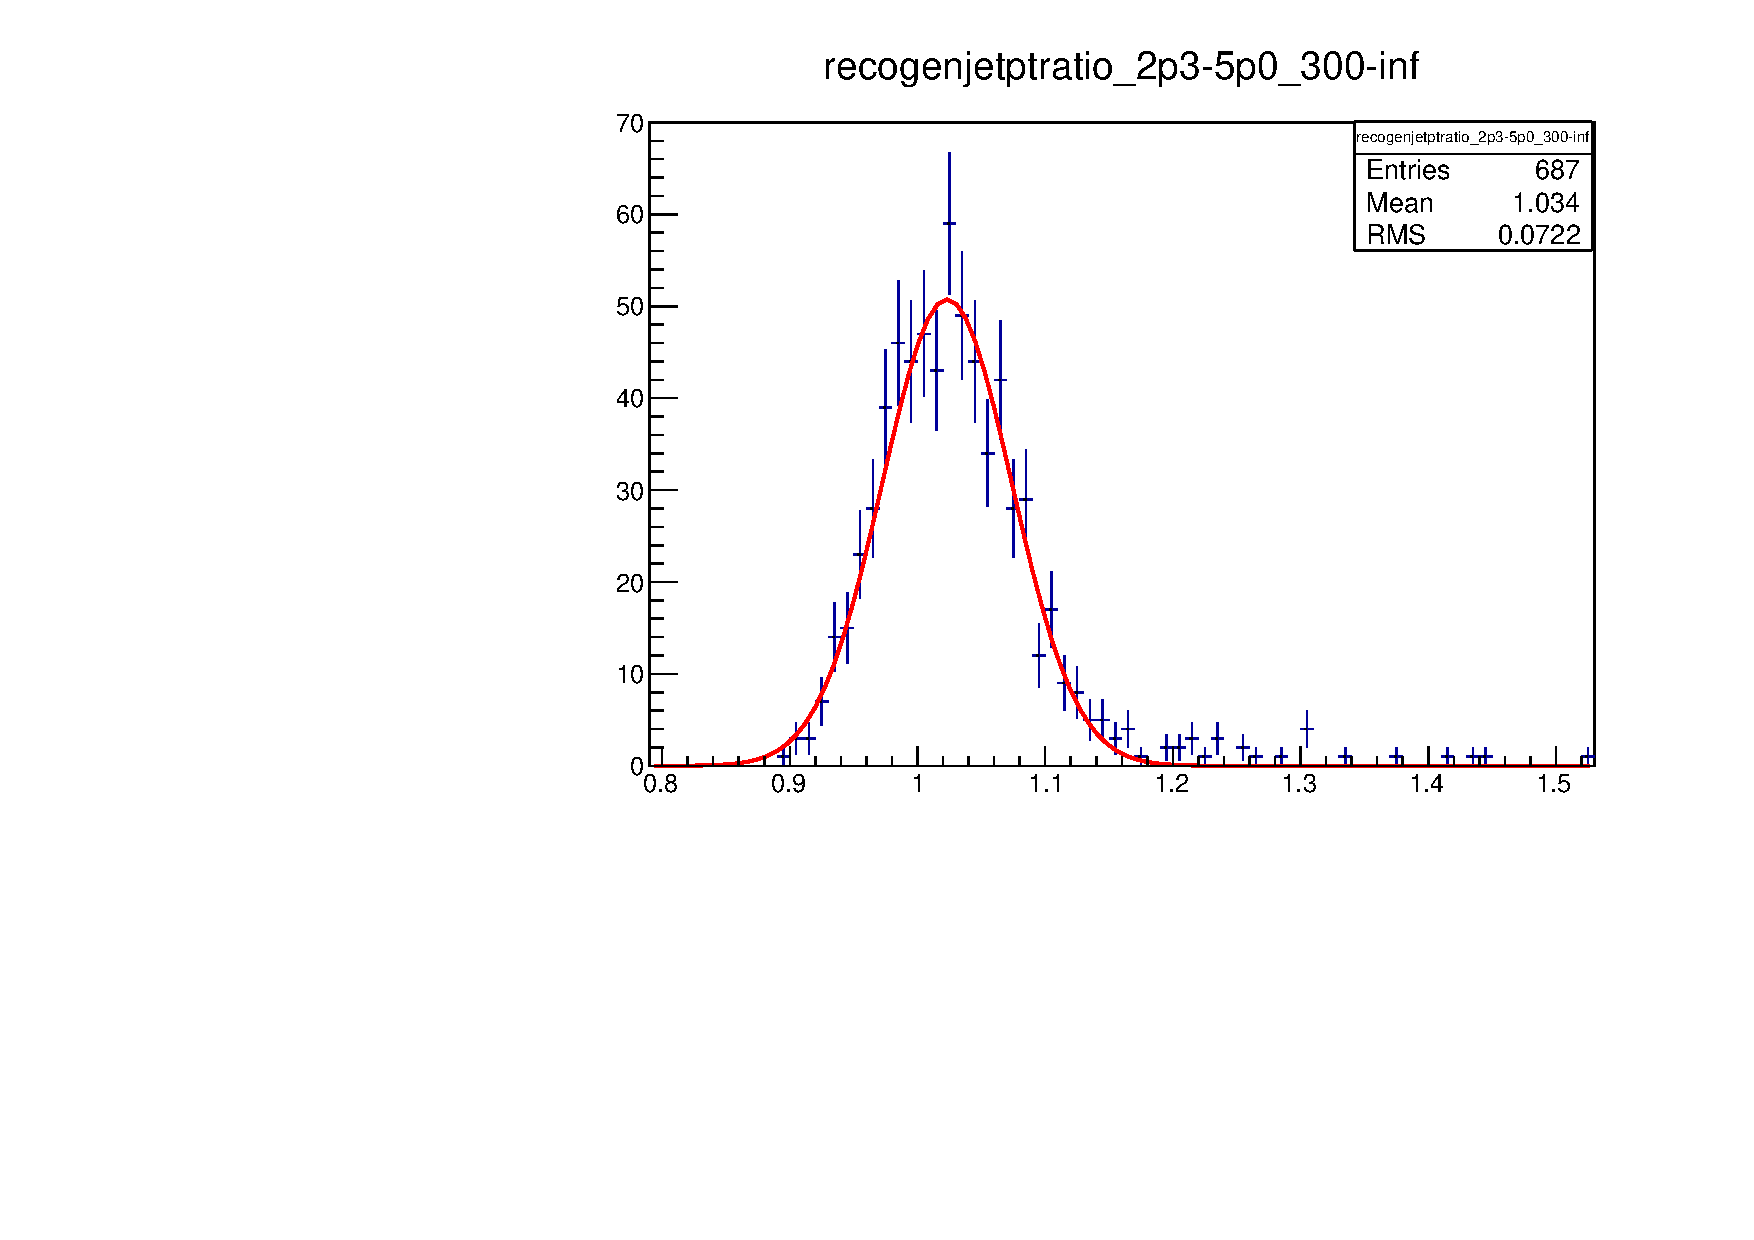
\includegraphics[width=1.1\textwidth]{TalkPics/jetres281013/Gausianfitplot.pdf}
  \end{columns}
\end{frame}

\begin{frame}
  \frametitle{Plots}
  \begin{center}
  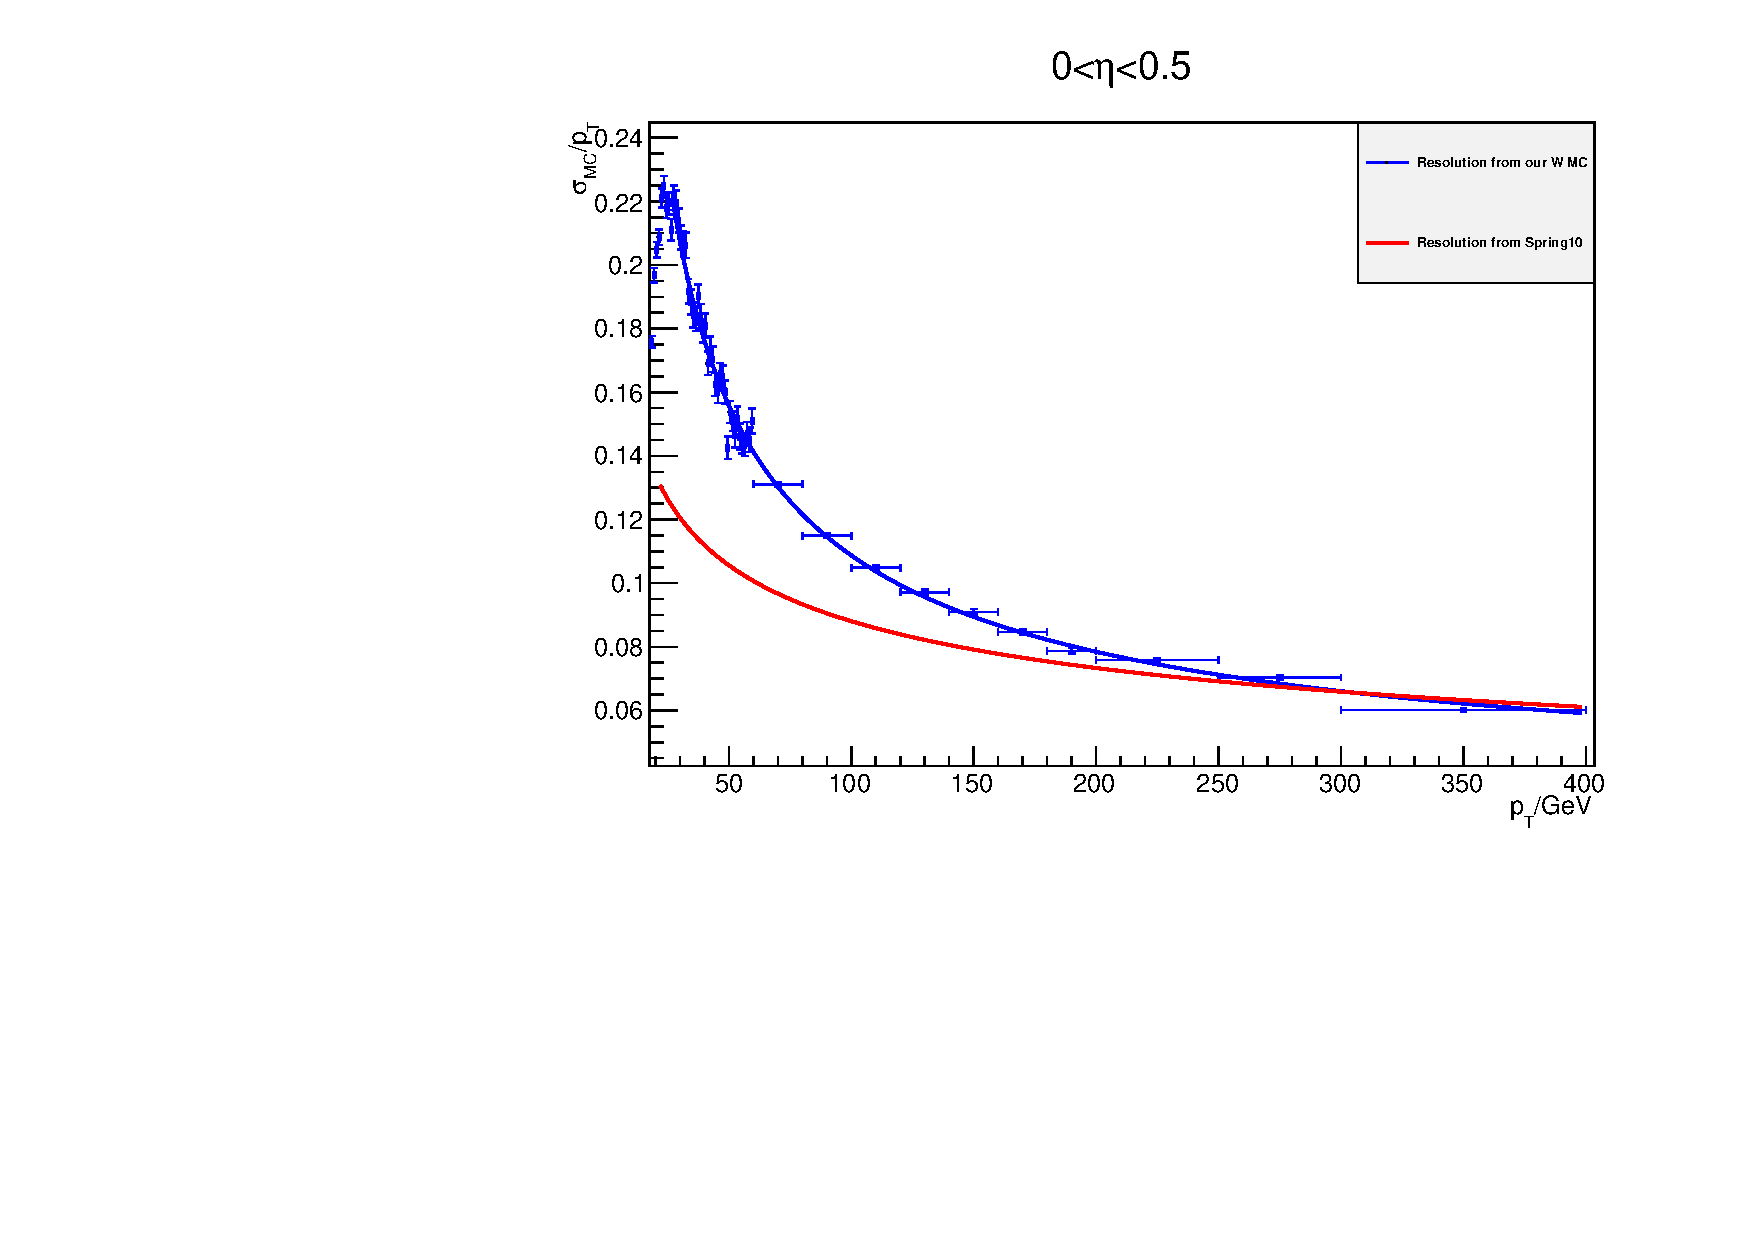
\includegraphics[width=.9\textwidth]{TalkPics/jetres281013/resforeta0p0-0p5.pdf}
  \end{center}
\end{frame}

\begin{frame}\label{lastframe}
  \frametitle{Plots}
  \begin{center}
  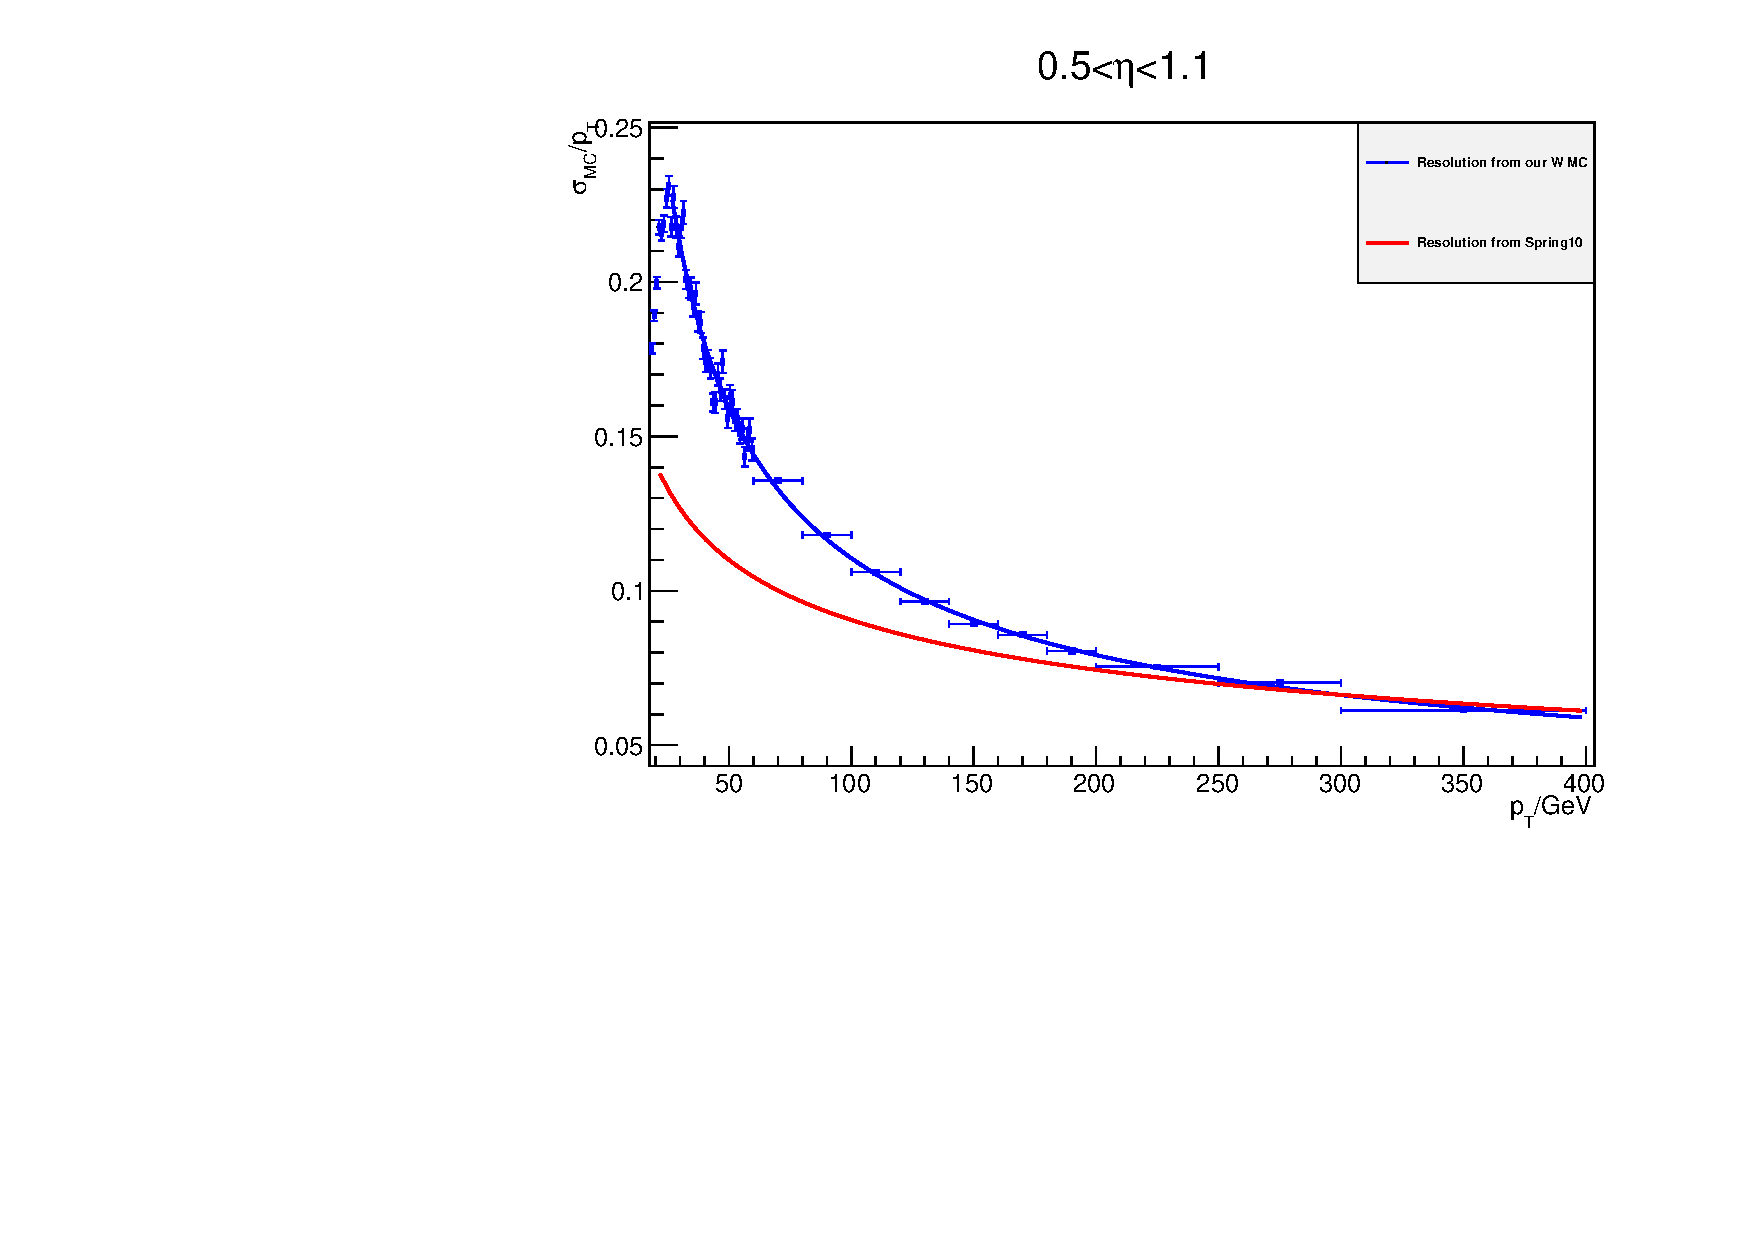
\includegraphics[width=.9\textwidth]{TalkPics/jetres281013/resforeta0p5-1p1.pdf}
  \end{center}
\end{frame}

\begin{frame}\label{lastframe}
  \frametitle{Plots}
  \begin{center}
  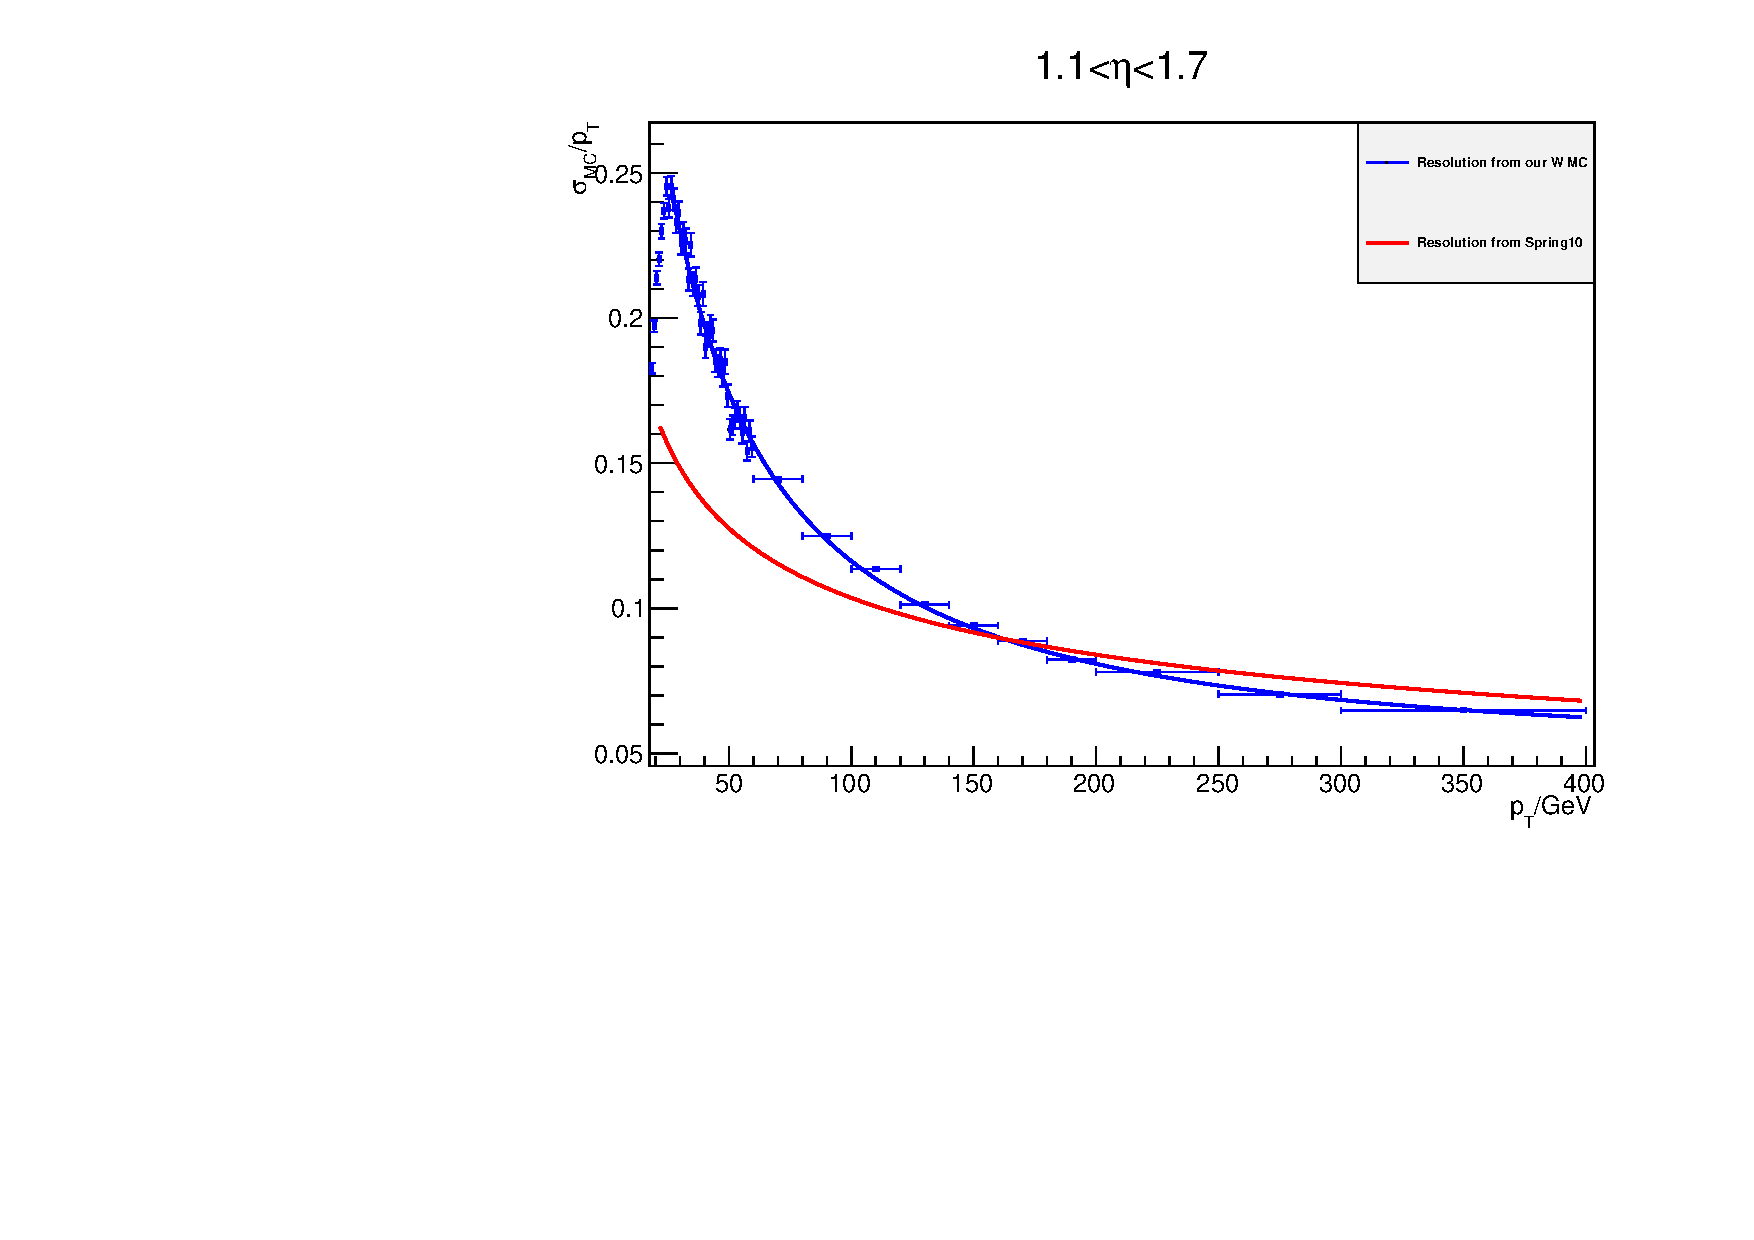
\includegraphics[width=.9\textwidth]{TalkPics/jetres281013/resforeta1p1-1p7.pdf}
  \end{center}
\end{frame}

\begin{frame}\label{lastframe}
  \frametitle{Plots}
  \begin{center}
  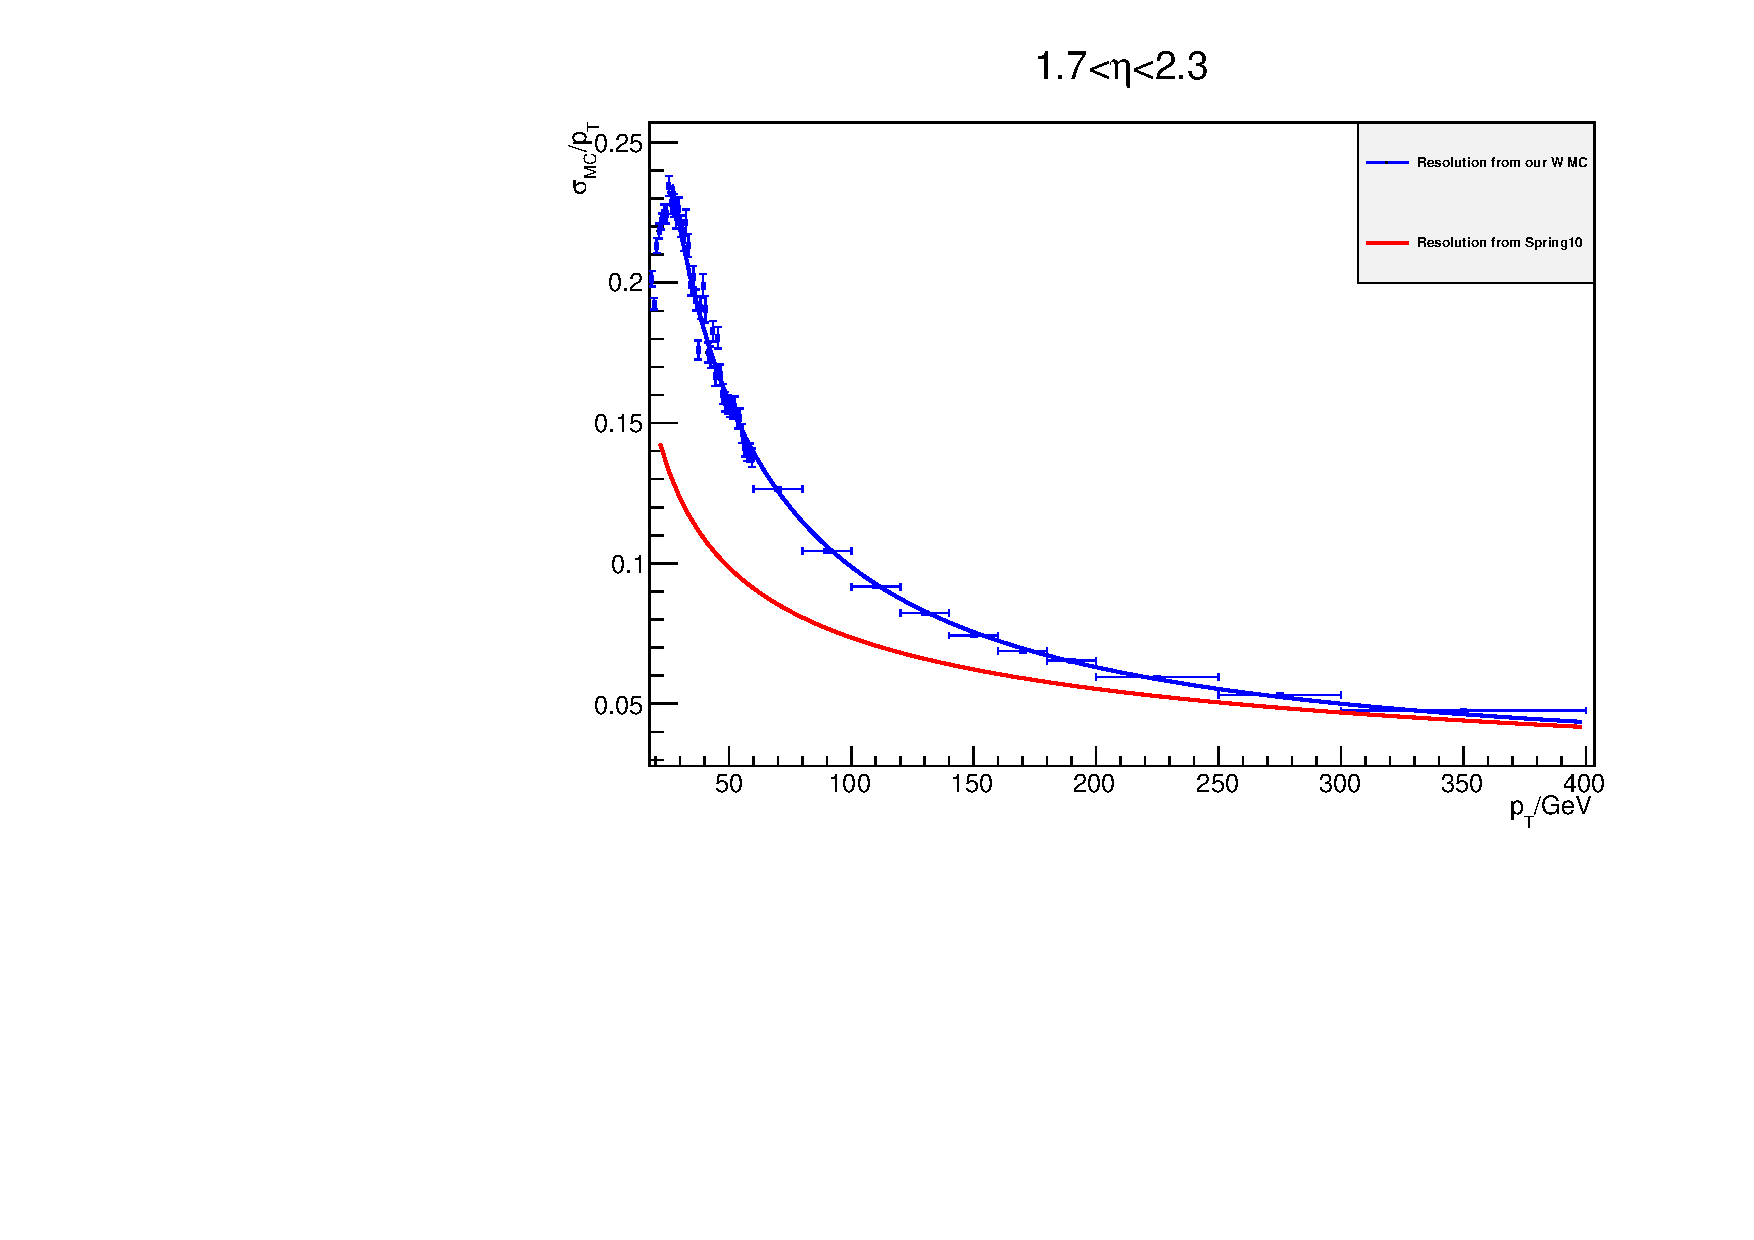
\includegraphics[width=.9\textwidth]{TalkPics/jetres281013/resforeta1p7-2p3.pdf}
  \end{center}
\end{frame}

\begin{frame}\label{lastframe}
  \frametitle{Plots}
  \begin{center}
  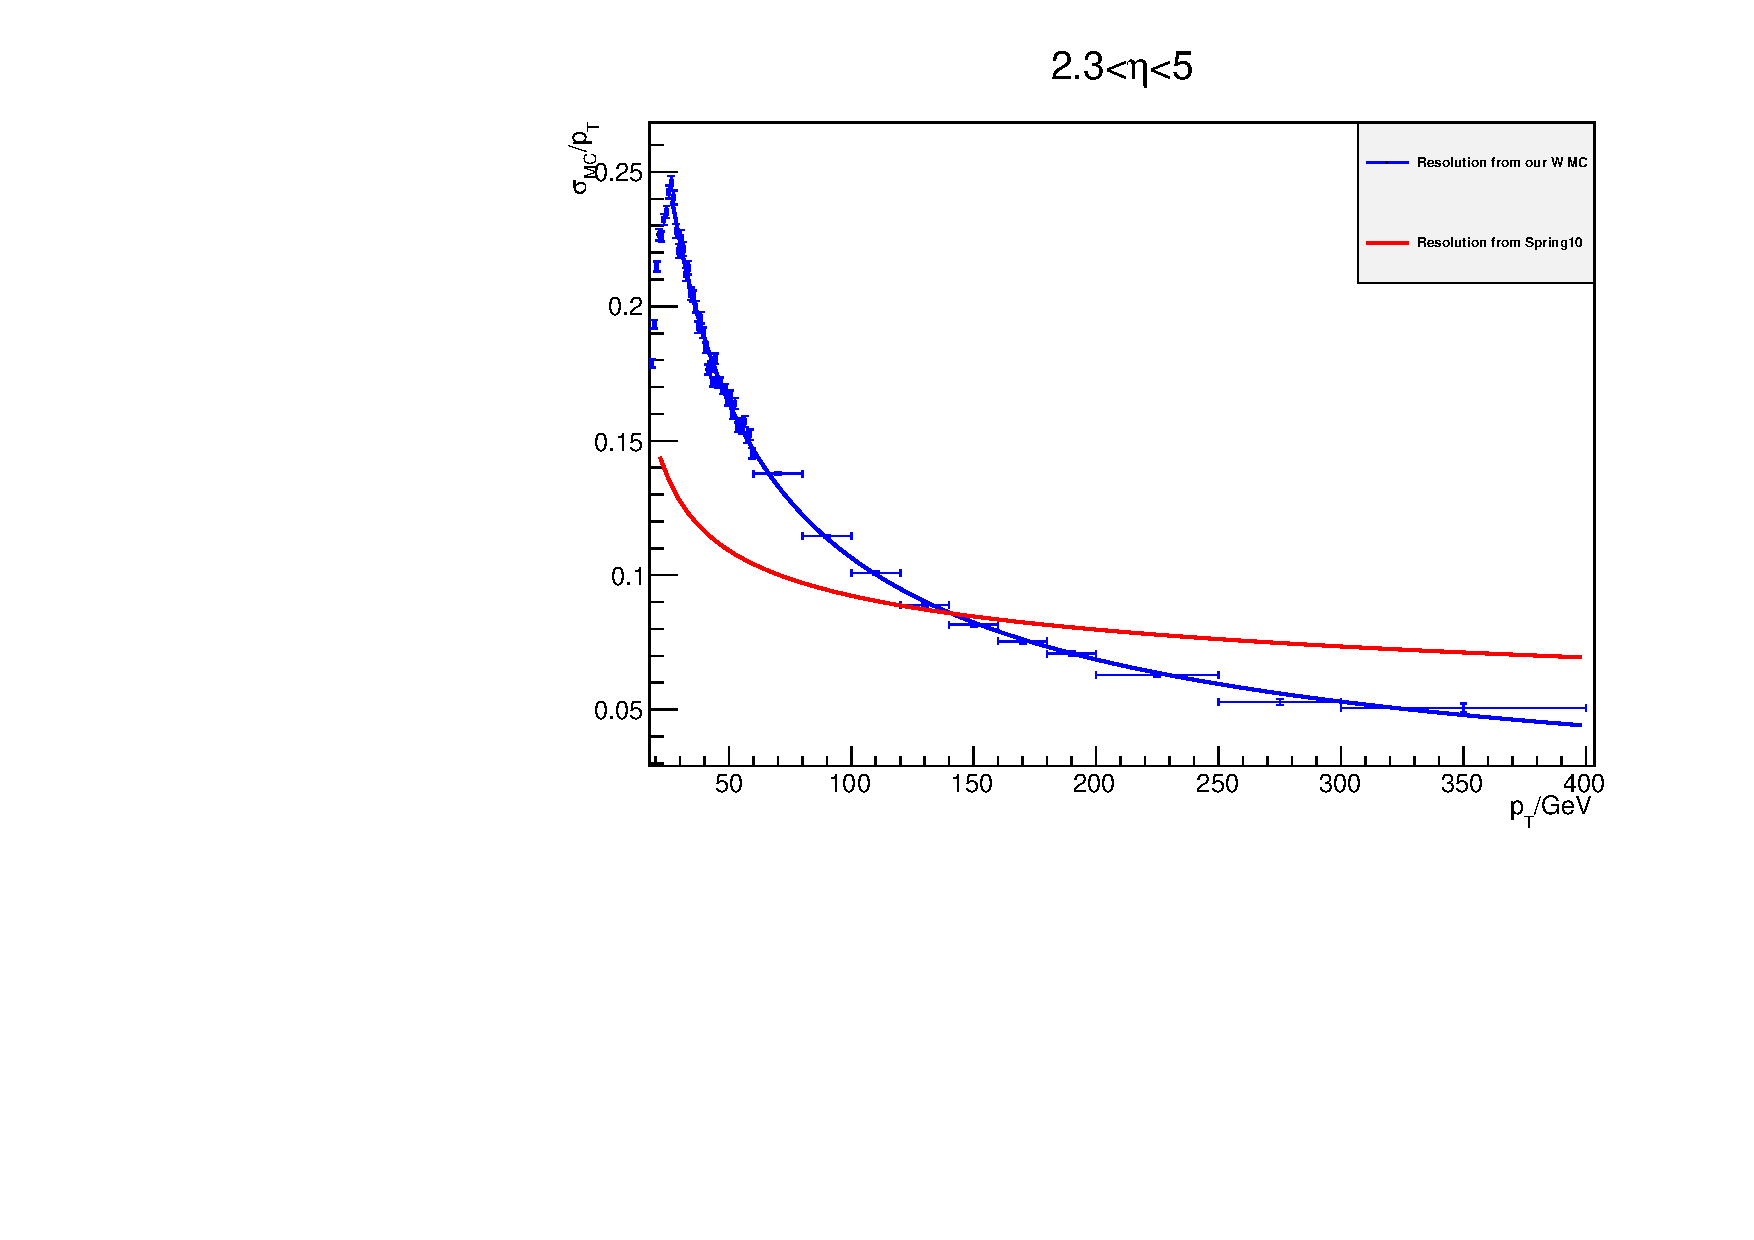
\includegraphics[width=.9\textwidth]{TalkPics/jetres281013/resforeta2p3-5p0.pdf}
  \end{center}
\end{frame}

\begin{frame}
  \frametitle{Turn on below 25 GeV}
  \begin{block}{}
    \footnotesize
  \begin{itemize}
  \item Clear turn on in MC below 25 GeV
  \item[-] 2010 JetMET paper plots only go down to 40 GeV
  \item[-] Spring 10 Resolutions do not have a turn on
  \item To produce results two methods have been used:
  \item[-] Fit resolution down to 25 GeV and treat as constant below 25 GeV
  \item[-] Fit resolution down to 20 GeV and extrapolate to below 20 GeV
  \end{itemize}
  \end{block}
\end{frame}

\begin{frame}
  \frametitle{Results}
  \begin{columns}
    \column{1.1\textwidth}
  \begin{block}{}
    \centering
    \footnotesize
    \begin{tabular}{|l|c|c|c|c|}
      \hline
      Channel & No gaussian & Spring 10 & Measured $\sigma_{MC}$ & Measured $\sigma_{MC}$ \\
      & smearing & $\sigma_{MC}$ & (flat below 25 GeV) & (extrapolate fit) \\
      \hline
      $W\rightarrow e \nu$ & 71.8 & 71.2 & 74.8 & 75.6 \\
      $W\rightarrow\mu\nu$ & 68.1 & 63.7 & 71.2 & 70.7 \\
      $W\rightarrow\tau\nu$ & 64.6 & 60.3 & 62.1 & 62.0 \\
      \hline
    \end{tabular}
  \end{block}
  \end{columns}
\end{frame}

\begin{frame}\label{lastframe}
  \frametitle{Conclusions}
  \begin{block}{}
    \footnotesize
  \begin{itemize}
  \item Gaussian smearing can make a significant difference to the final result
  \item[-] $|p_{T reco}-p_{T gen}|<3\sigma_{MC}$ matching condition used by runmetuncertainty is not implemented in analysis B
  \item The resolutions used by runmetuncertainty are very different to those in our MC especially at CJV and 50 GeV thresholds
  \end{itemize}
  \end{block}
\end{frame}

\end{fmffile}
\end{document}
